\documentclass[pdflatex,compress]{beamer}

%\usetheme[dark,framenumber,totalframenumber]{ElektroITK}
\usetheme[darktitle,framenumber,totalframenumber]{ElektroITK}

\usepackage{graphicx}

\title{PEMODELAN JARINGAN KOMUNIKASI}
\subtitle{OSI Layer 4 - The Transport Layer}

\author{Mifta Nur Farid, S.T., M.T.}

\begin{document}

\maketitle

\begin{frame}
	\frametitle{Layer 4 - The Transport Layer}
	\begin{itemize}
		\item The Transport layer provides transparent transfer of data between hosts and is responsible for end-to-end error recovery and flow control.
		\item Flow control is the process of adjusting the flow of data from the sender to ensure that the receiving host can handle all of it.
	\end{itemize}
\end{frame}

\begin{frame}
	\frametitle{Session Multiplexing}
	\begin{itemize}
		\item Session multiplexing is the process by which a host is able to support multiple sessions simultaneously and manage the individual traffic streams over a single link.
	\end{itemize}
	\begin{center}
		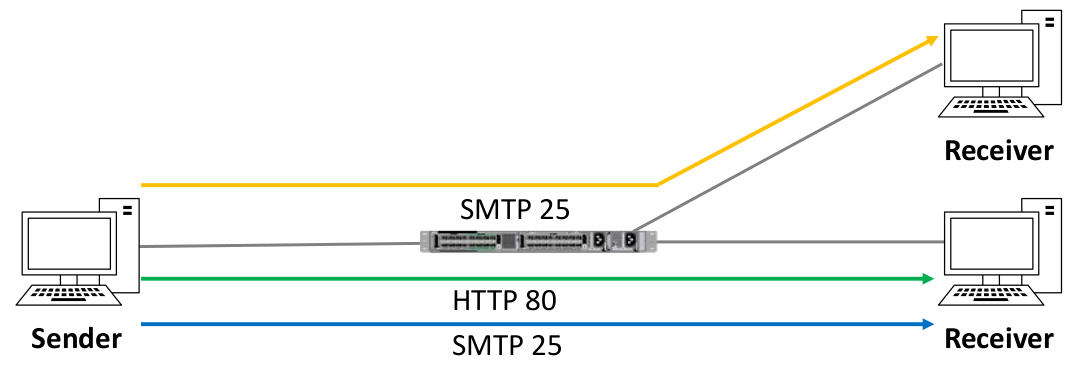
\includegraphics[width=\linewidth]{img/img01}
	\end{center}
\end{frame}

\begin{frame}
	\frametitle{Layer 4 Port Numbers}
	\begin{itemize}
		\item The Layer 4 destination port number is used to identify the upper layer protocol.
		\item For example, HTTP uses port 80, SMTP email uses port 25.
		\item The sender also adds a source port number to the Layer 4 header.
		\item The combination of source and destination port number can be used to track sessions.
	\end{itemize}
	\begin{center}
		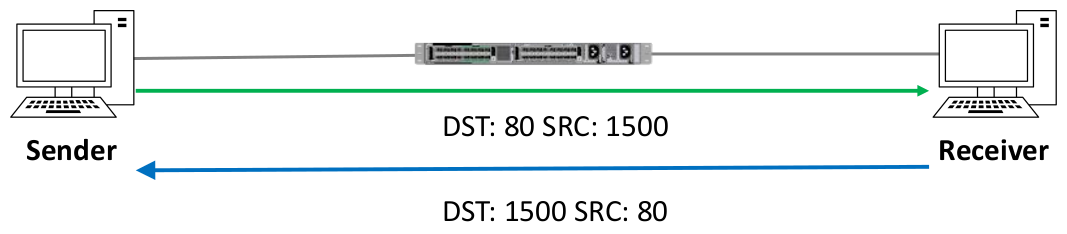
\includegraphics[width=\linewidth]{img/img02}
	\end{center}
\end{frame}

\begin{frame}
	\frametitle{Transport Control Protocol (TCP)}
	\begin{itemize}
		\item TCP (Transport Control Protocol) and UDP (the User Datagram Protocol) are the most common Layer 4 protocols.
		\item TCP is connection oriented - once a connection is established, data can be sent bidirectionally over that connection.
		\item TCP carries out sequencing to ensure segments are processed in the correct order and none are missing.
		\item TCP is reliable - the receiving host sends acknowledgments back to the sender. Lost segments are resent.
		\item TCP performs flow control.
	\end{itemize}
\end{frame}

\begin{frame}
	\frametitle{The TCP Three-Way Handshake}
	\begin{center}
		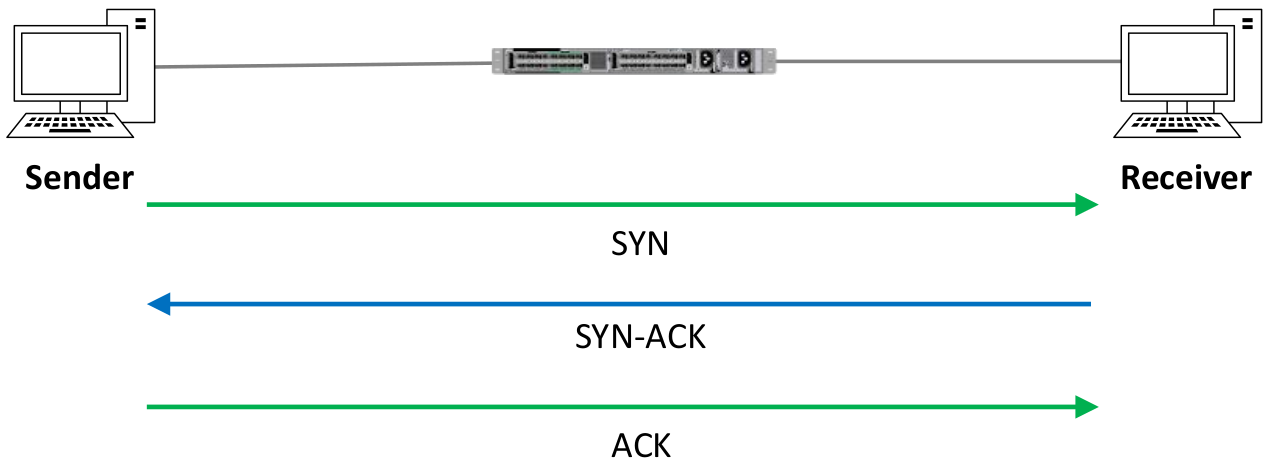
\includegraphics[width=\linewidth]{img/img03}
	\end{center}
\end{frame}

\begin{frame}
	\frametitle{OSI Reference Model - Encapsulation}
	\begin{center}
		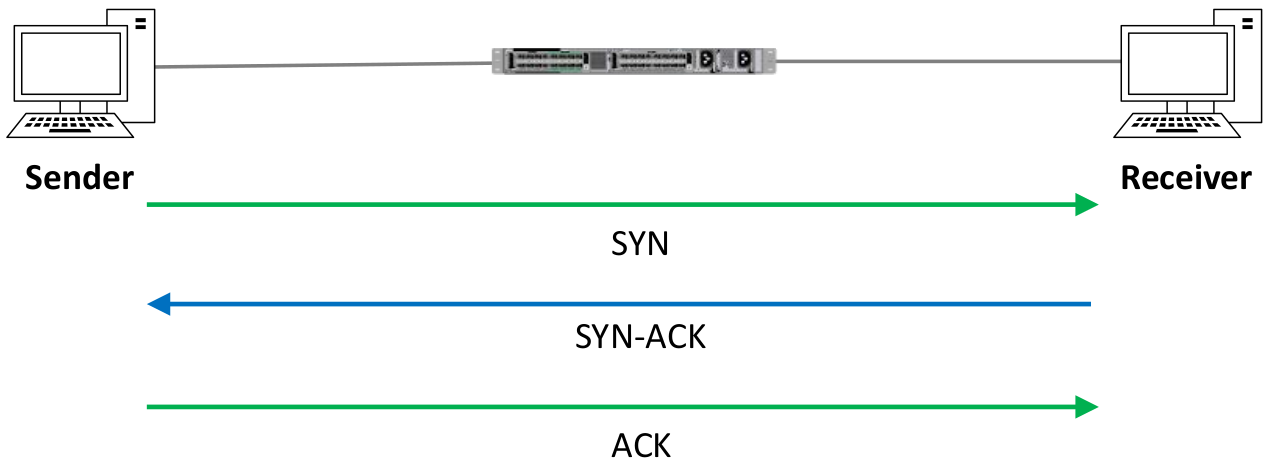
\includegraphics[width=\linewidth]{img/img03}
	\end{center}
\end{frame}

\begin{frame}
	\frametitle{OSI Reference Model - Encapsulation}
	\begin{center}
		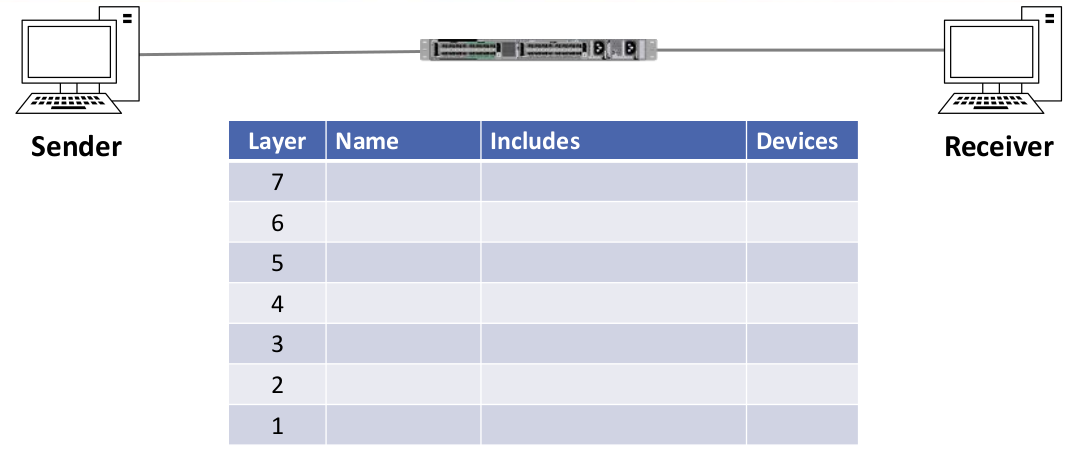
\includegraphics[width=\linewidth]{img/img04}
	\end{center}
\end{frame}

\begin{frame}
	\frametitle{OSI Reference Model - Encapsulation}
	\begin{center}
		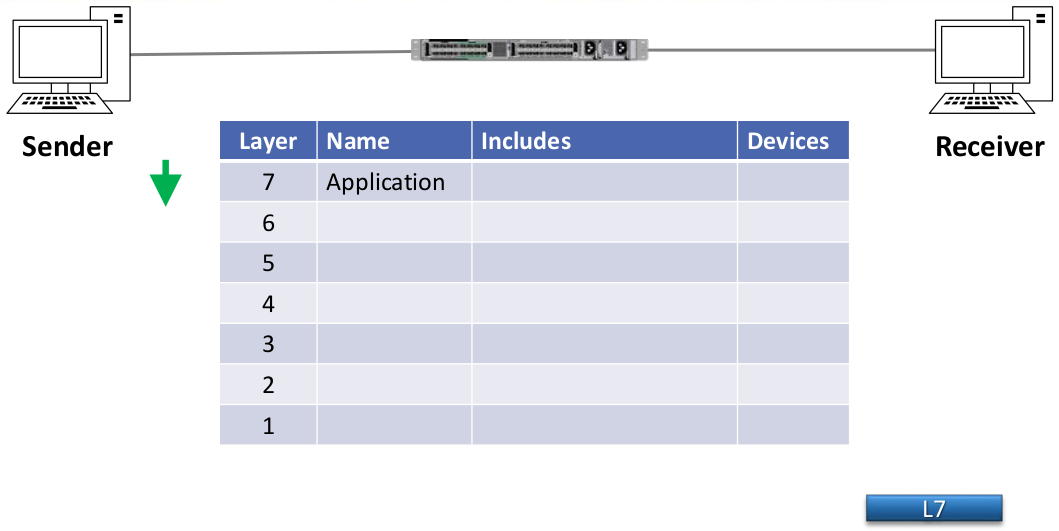
\includegraphics[width=\linewidth]{img/img05}
	\end{center}
\end{frame}

\begin{frame}
	\frametitle{OSI Reference Model - Encapsulation}
	\begin{center}
		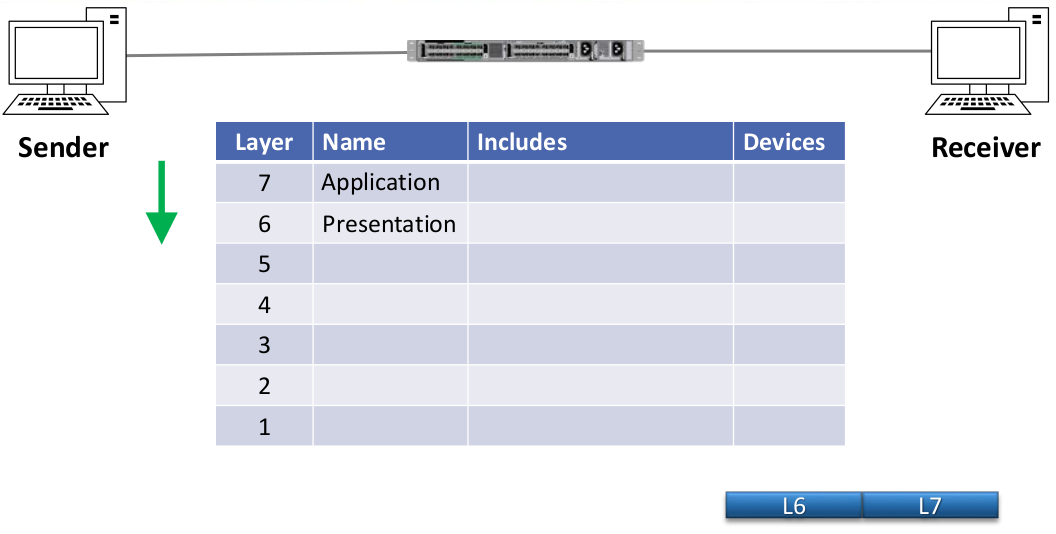
\includegraphics[width=\linewidth]{img/img06}
	\end{center}
\end{frame}

\begin{frame}
	\frametitle{OSI Reference Model - Encapsulation}
	\begin{center}
		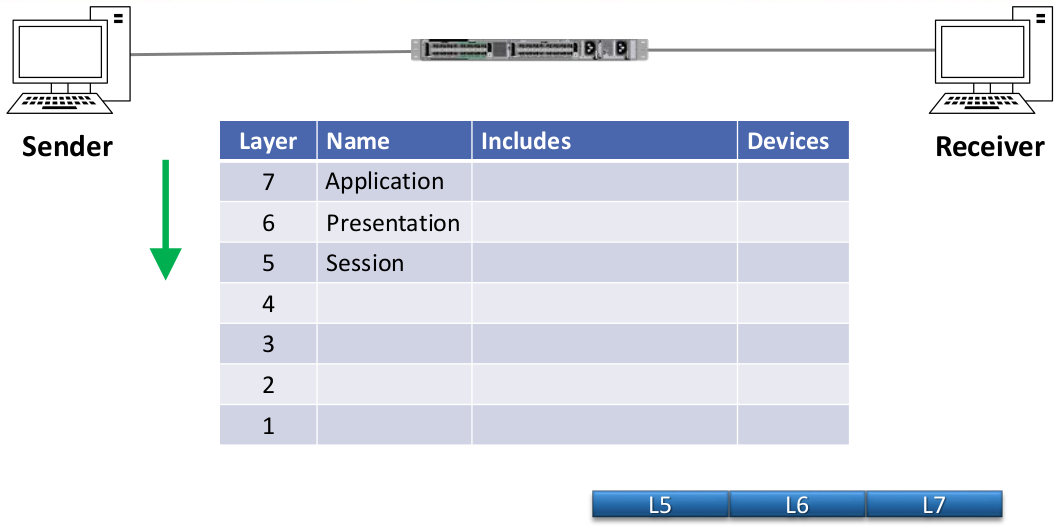
\includegraphics[width=\linewidth]{img/img07}
	\end{center}
\end{frame}

\begin{frame}
	\frametitle{OSI Reference Model - Encapsulation}
	\begin{center}
		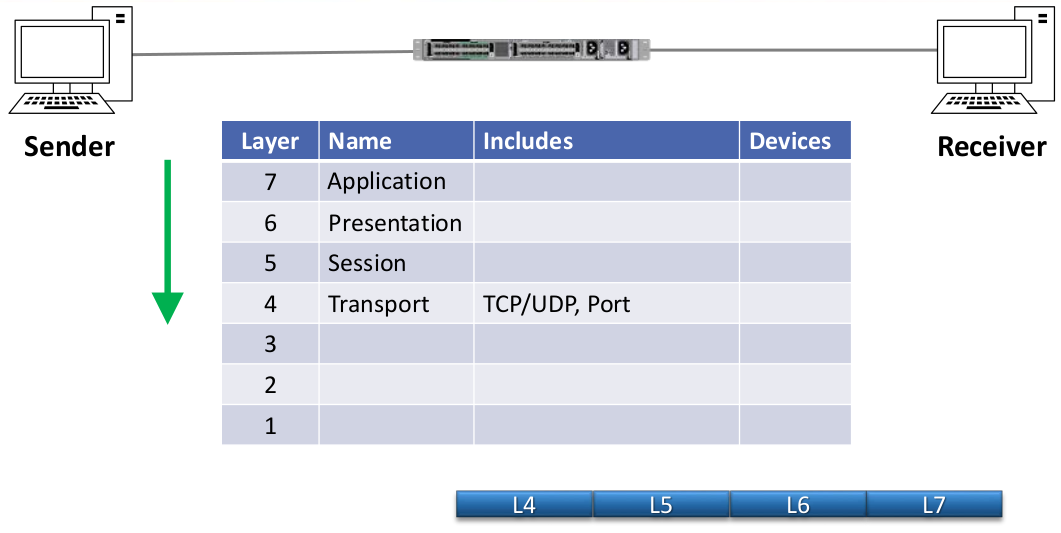
\includegraphics[width=\linewidth]{img/img08}
	\end{center}
\end{frame}

\begin{frame}
	\frametitle{OSI Reference Model - Encapsulation}
	\begin{center}
		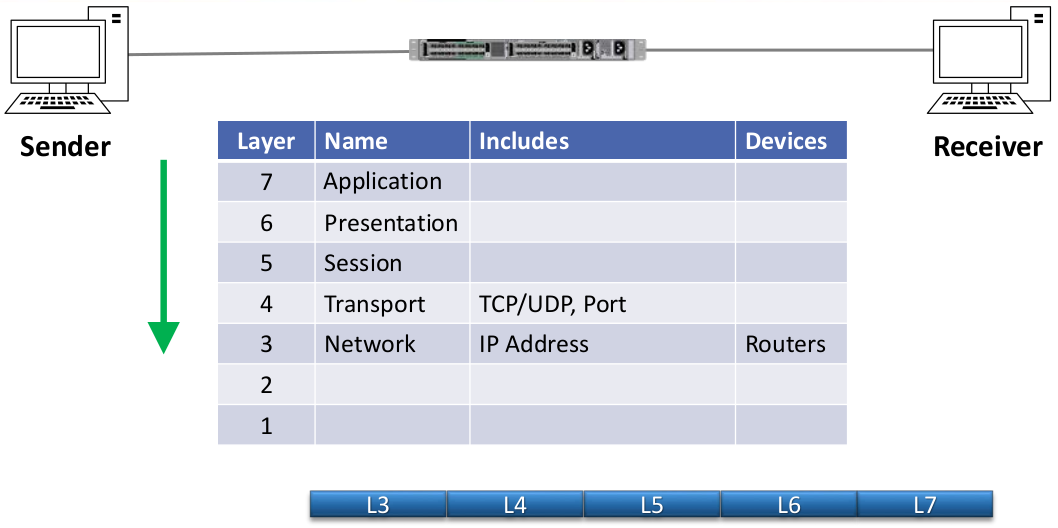
\includegraphics[width=\linewidth]{img/img09}
	\end{center}
\end{frame}

\begin{frame}
	\frametitle{OSI Reference Model - Encapsulation}
	\begin{center}
		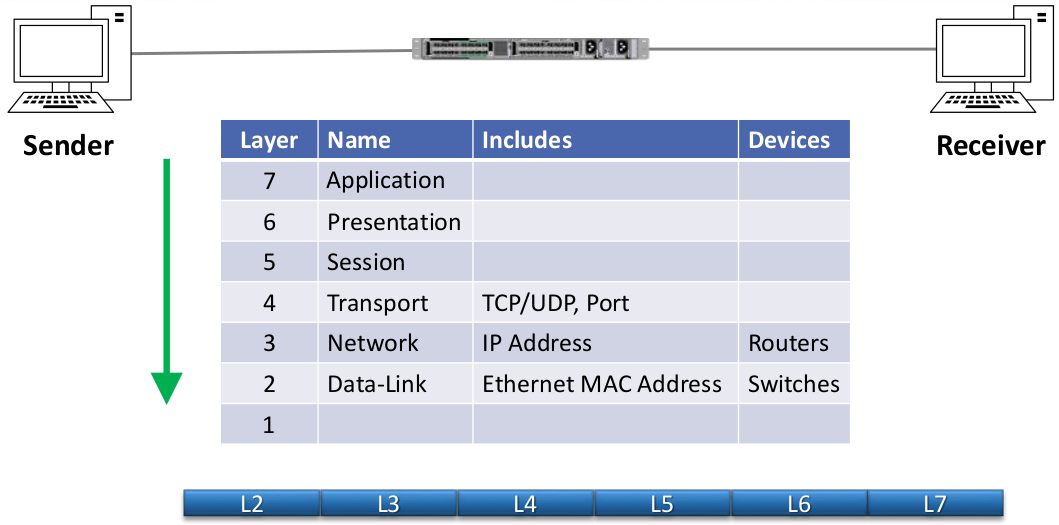
\includegraphics[width=\linewidth]{img/img10}
	\end{center}
\end{frame}

\begin{frame}
	\frametitle{OSI Reference Model - Encapsulation}
	\begin{center}
		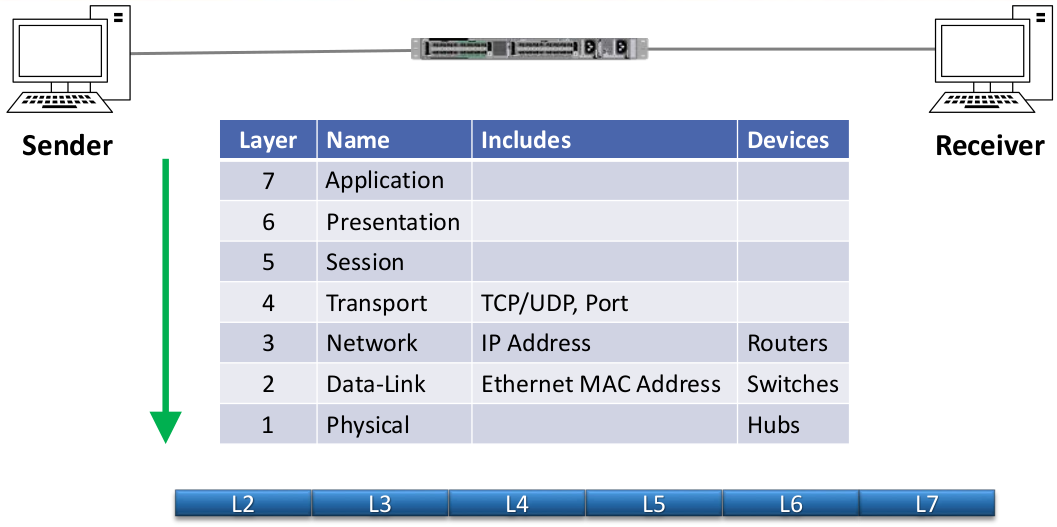
\includegraphics[width=\linewidth]{img/img11}
	\end{center}
\end{frame}

\begin{frame}
	\frametitle{The TCP Header}
	\begin{center}
		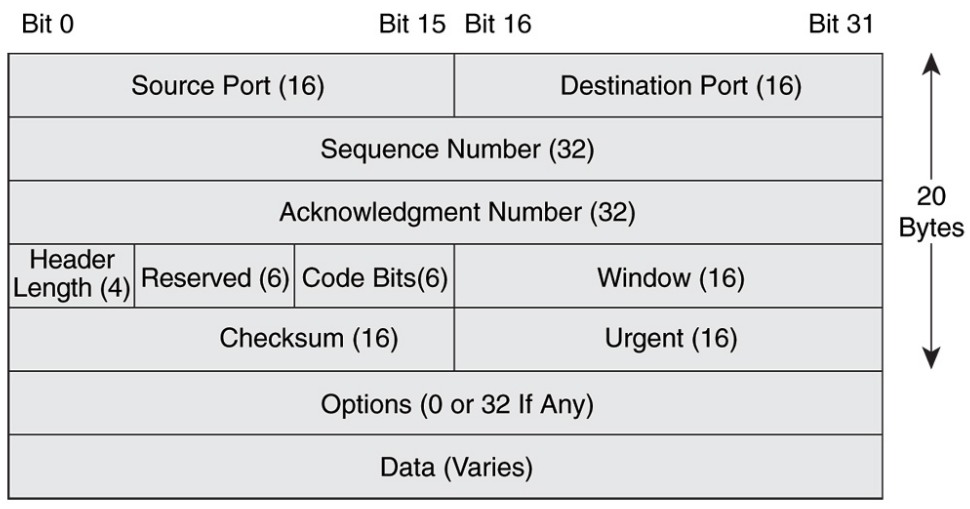
\includegraphics[width=\linewidth]{img/img12}
	\end{center}
\end{frame}

\begin{frame}
	\frametitle{User Datagram Protocol (UDP)}
	\begin{itemize}
		\item The User Datagram Protocol sends traffic best effort.
		\item UDP is not connection oriented. There is no handshake connection setup between the hosts.
		\item UDP does not carry out sequencing to ensure segments are processed in the correct order and none are missing.
		\item UDP is not reliable – the receiving host does not send acknowledgments back to the sender.
		\item UDP does not perform flow control.
		\item If error detection and recovery is required it is up to the upper layers to provide it.
	\end{itemize}
\end{frame}

\begin{frame}
	\frametitle{The UDP Header}
	\begin{center}
		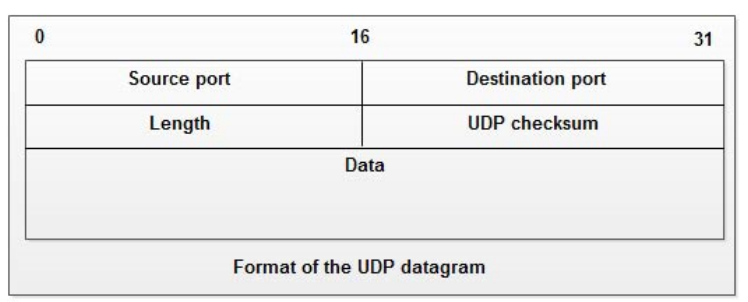
\includegraphics[width=\linewidth]{img/img13}
	\end{center}
\end{frame}

\end{document}